\documentclass[dvipdfmx,12pt,a4paper]{jreport}
	\usepackage{geometry}
    \usepackage{pdfpages}
    \usepackage{graphicx}
    \usepackage{newtxmath}
    \usepackage{array}
    \usepackage{siunitx}
    \usepackage{url}
    \usepackage{amsmath}
    \usepackage{comment}
    \usepackage{amsfonts}
		\usepackage{bm}
    \usepackage{here}
    \geometry{left=20mm,right=20mm,top=25mm,bottom=25mm} %geometry:余白設定
    \renewcommand{\bibname}{参考文献}
    %\renewcommand{\figurename}{Fig.}
    %\renewcommand{\tablename}{Tab.}
    \makeatletter
    \DeclareRobustCommand\cite{\unskip
    	\@ifnextchar[{\@tempswatrue\@citex}{\@tempswafalse\@citex[]}}
    \def\@cite#1#2{$^{\hbox{\scriptsize{[#1\if@tempswa , #2\fi}]}}$}
    \def\@biblabel#1{[#1]}
    \makeatother
    
    \graphicspath{{./graphics/}} %図のディレクトリを設定.フォルダの場所によって先頭' . 'の数を変える.
\begin{document}
	\begin{titlepage}
		
		\begin{center}
			
			\vspace{20truept}
			{\LARGE 2022年度}\\
			\vspace{15truept}
			{\LARGE 修士論文}
			
			\vspace{50truept}
			
			{\Huge Silk Fibroin Filmの圧電性向上の研究}\\
			\vspace{10truept}
			
			\vspace*{280truept}
			
			{\LARGE 1521516}\\
			\vspace{5truept}
			
			{\LARGE 金木 進}\\
			\vspace{60truept}
			
			{\LARGE 2023年3月}
			\vspace{30truept}
			
			{\LARGE 東京理科大学}\\
			\vspace{15truept}
			
			{\LARGE 理学研究科 応用物理学専攻}\\
			\vspace{15truept}
			
			{\LARGE 中嶋研究室}\\
			
		\end{center}
		
		
	\end{titlepage}
  \thispagestyle{empty}
	\clearpage
\addtocounter{page}{0}
\tableofcontents
  \chapter{序論}
		\section{研究背景}
		\subsection{SDGs}
		2015年9月25日-27日、国連総会において「国連持続可能な開発サミット」
		が開催された。そして、2030年までに実現する国際目標として
		 "Transforming Our World: 2030 Agenda for Sustainable Development" が採択された\cite{sdgs_2030}。
		だれも取り残さなさい(leave no one behind)を基本理念とし、
		17の目標と169のターゲットから構成されている。まとめて
		「持続可能な開発目標(SDGs: Sustainable Development Goals)」と呼ばれる。
		図\ref{sdgs_poster}の通り、17個の目標は貧困、紛争、健康などの人間的な活動の問題から
		気候変動、海洋環境など環境問題まで言及している。
		科学技術の向上により人類の生活は向上してきたが、今後は環境に対する負荷、
		発展途上国にも普及するか、なども考慮しなくてはならない。
		\\
		\\

		\begin{figure}[h]
			\centering
			
\includegraphics[width=\linewidth]{sdgs_poster.jpg}
			\caption{持続な開発目標(SDGs)における17個の目標が記述されたポスター\cite{sdgs_poster}}
			\label{sdgs_poster}
		\end{figure}
		\newpage
		\subsection{絹糸}
		\section{研究の目的}

	\chapter{原理}
		\section{圧電性}
		\subsection{圧電基本式}
		圧電体には正圧電効果と逆圧電効果という性質が存在する。
		生じた歪みに対して、応力と電場の寄与がある。
		さらに生じた電束密度に対しても電場と歪みの二つの寄与がある。
		これらを式にまとめると
				\begin{eqnarray}
					\begin{cases}
						\delta S=\frac{\partial S}{\partial T}\delta T + \frac{\partial S}{\partial E} \delta E 
						= s^{E}\delta T+d \delta E & \\
						\delta D=\frac{\partial D}{\partial T}\delta T + \frac{\partial D}{\partial E}\delta E 
						= d \delta T+\varepsilon^T \delta E  &
					\end{cases}
					\label{圧電d形式1}
				\end{eqnarray}
			となる。実際の試料は1軸方向、2軸方向、3軸方向のみだけでなく、
			せん断歪みを考慮する必要があり、テンソル形式で記述される。
			ここで、$\delta S\rightarrow S, \delta T\rightarrow T,
			\delta E\rightarrow E, \delta D\rightarrow D$とし、テンソル行列を$\left[ \right]$で表すと
			式\ref{圧電d形式1}は
			\begin{equation}
				\begin{cases}
					\left[S\right]=\left[s^E\right]\left[T\right]+\left[d_t\right]\left[E\right]& \\
					\left[D\right]=\left[d\right]\left[T\right]+\left[\varepsilon^T\right]\left[E\right]
				\end{cases}
				\label{圧電d形式2}
			\end{equation}
			となり、これを圧電d形式と呼ぶ。
			式\ref{圧電d形式2}をテンソルの要素も含めて記述すると
			\begin{equation}
				\begin{cases}
				\left(
				\begin{array}{c}
					S_1 \\
					S_2 \\
					S_3 \\
					S_4 \\
					S_5 \\
					S_6 
				\end{array}
				\right)=\left(
				\begin{array}{cccccc}
				s^E_{11} & s^E_{12} & s^E_{13} & s^E_{14} & s^E_{15} & s^E_{16} \\
				s^E_{21} & s^E_{22} & s^E_{23} & s^E_{24} & s^E_{25} & s^E_{26} \\
				s^E_{31} & s^E_{32} & s^E_{33} & s^E_{34} & s^E_{35} & s^E_{36} \\
				s^E_{41} & s^E_{42} & s^E_{43} & s^E_{44} & s^E_{45} & s^E_{46} \\
				s^E_{51} & s^E_{52} & s^E_{53} & s^E_{54} & s^E_{55} & s^E_{56} \\
				s^E_{61} & s^E_{62} & s^E_{63} & s^E_{64} & s^E_{65} & s^E_{66} \\
				\end{array}
				\right)
				\left(
				\begin{array}{c}
					T_1 \\
					T_2 \\
					T_3 \\
					T_4 \\
					T_5 \\
					T_6 
				\end{array}
				\right)+
				\left(
				\begin{array}{ccc}
					d_{11} & d_{21}	& d_{31} \\
					d_{12} & d_{22}	& d_{32} \\
					d_{13} & d_{32}	& d_{33} \\
					d_{14} & d_{42} & d_{34} \\
					d_{15} & d_{52} & d_{35} \\
					d_{16} & d_{62}	& d_{36}
				\end{array}
				\right)
				\left(
				\begin{array}{c}
					E_1 \\
					E_2 \\
					E_3 \\
				\end{array}
				\right) & \\
				\left(
				\begin{array}{c}
					D_1 \\
					D_2 \\
					D_3
				\end{array}\right)=\left(
				\begin{array}{cccccc}
					d_{11} & d_{12} & d_{13} & d_{14} & d_{15} & d_{16} \\
					d_{21} & d_{22} & d_{23} & d_{24} & d_{25} & d_{26} \\
					d_{31} & d_{32} & d_{33} & d_{34} & d_{35} & d_{36}
				\end{array}\right)
				\left(
				\begin{array}{c}
					T_1 \\
					T_2 \\
					T_3 \\
					T_4 \\
					T_5 \\
					T_6 
				\end{array}
				\right)+\left(
				\begin{array}{ccc}
					\varepsilon^T_{11}&0&0 \\
					0&\varepsilon^T_{11}&0 \\
					0&0&\varepsilon^T_{33}
				\end{array}\right)
				\left(
				\begin{array}{c}
					E_1 \\
					E_2 \\
					E_3 \\
				\end{array}\right)
				\end{cases}
			\end{equation}
			となる。式\ref{圧電d形式2}を式変形すると
			\begin{equation}
				\begin{cases}
				\left[T\right]=\left[c^E\right]\left[S\right]-\left[e_t\right]\left[E\right] & \\
				\left[D\right]=\left[e\right]\left[S\right]+\left[\varepsilon^S\right]\left[E\right]
				\end{cases}
				\label{圧電e形式}
			\end{equation}
			\begin{equation}
				\begin{cases}
					\left[S\right]=\left[s^D\right]\left[T\right]-\left[g_t\right]\left[D\right] & \\
					\left[E\right]=-\left[g\right]\left[T\right]+\left[\beta^T\right]\left[D\right]
				\end{cases}
				\label{圧電g形式}
			\end{equation}
			\begin{equation}
				\begin{cases}
					\left[T\right]=\left[c^D\right]\left[S\right]-\left[h_t\right]\left[D\right] & \\
					\left[E\right]=-\left[h\right]\left[S\right]+\left[\beta^s\right]\left[D\right]
				\end{cases}
				\label{圧電h形式}
			\end{equation}
			の三式を導け、それぞれ式\ref{圧電e形式}を圧電e形式, 
			式\ref{圧電g形式}を圧電g形式, 式\ref{圧電h形式}を圧電h形式と呼ぶ。応力$T$, 電場$E$, 歪み$S$, 電束密度$D$の係数である$[d],[e],[g],[h]$ではそれぞれ、
			\begin{equation}
				d_{ij}=\left(\frac{\partial D_i}{\partial T_j}\right)_E=\left(\frac{\partial S_j}{\partial E_i}\right)_T
			\end{equation}
			\begin{equation}
				e_{ij}=\left(\frac{\partial D_i}{\partial S_j}\right)_E=-\left(\frac{\partial T_j}{\partial E_i}\right)_S
			\end{equation} 
			\begin{equation}
				g_{ij}=-\left(\frac{\partial E_i}{\partial T_j}\right)_D=\left(\frac{\partial S_j}{\partial D_i}\right)_T
			\end{equation}
			\begin{equation}
				h_{ij}=-\left(\frac{\partial E_i}{\partial S_j}\right)_D=-\left(\frac{\partial T_j}{\partial D_i}\right)_S
			\end{equation}
			で定義される。また、それぞれの圧電定数間には弾性コンプライアンス$s$、
			誘電率$\varepsilon$を介して以下の関係がある。
			\begin{equation}
				d = e s
			\end{equation}
			\begin{equation}
				g = h s
			\end{equation}
			\begin{equation}
				d = \varepsilon g
			\end{equation}
			\begin{equation}
				e = \varepsilon h
			\end{equation}
			\subsection{電気機械結合係数}
			物理変数が異なる系の物理変数を変化させる現象を結合効果という。
			力や温度変化によって分極が変化する現象はそれぞれ圧電効果(piezoelectric effect)
			及び焦電効果(pyroelectric effect)と呼ばれる。

			\begin{figure}[h]
				\centering
				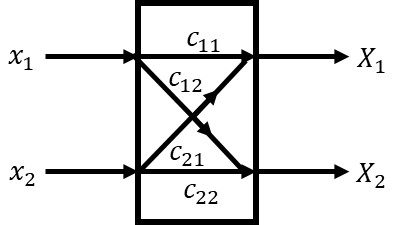
\includegraphics{結合効果.jpg}
				\caption{結合効果}
				\label{結合効果}
			\end{figure}
			図\ref{結合効果}のように2種類の共役な物理変数 ($x_1$, $X_1$),($x_2$, $X_2$)
			について、その間に線形な結合があると、熱力学ポテンシャルは、一般化したひずみ $x$ を独立変数として
			\begin{equation}
				\Phi=\frac{1}{2}c_{11}x_1^2 + c_{12}x_1x_2+\frac{1}{2}c_{22}x_2^2
			\end{equation}
			と書ける。$x$に共役した力$X$は
			\begin{equation}
				X_1 = \left( \frac{\partial \Phi}{\partial x_1} \right)_{x_2} = c_{11}x_1+c_{12}x_2
			\end{equation}
			\begin{equation}
				X_2 = \left( \frac{\partial \Phi}{\partial x_2} \right)_{x_1} = c_{12}x_1 + c_{22}x_2
			\end{equation}
			となり、係数 $c_{12}$を介して異なる物理変数への結合が起きることが分かる。
			非線形な結合である場合も線形な場合と同様の上式2つで記述できる。
			両方向の結合の係数が等しく、これを相反定理($c_{12}=c_{21}$)という。
			また、異なる系の間におけるエネルギー変換効率として結合系数$k$を式\ref{結合係数}のように定義する。
			\begin{equation}
				k^2=\frac{c_{12}^2}{c_{11}c_{22}}
				\label{結合係数}
			\end{equation}
			
			\begin{comment}
			圧電定数と同様に、圧電効果を示す定数として電気機械結合係数$k$がある。
			電気機械結合係数$k$は電気的エネルギーと機械的エネルギーの変換を表す係数であり、
			式\ref{電気機械結合係数の定義}のように与えた電気エネルギーと生じた機械エネルギー、
			あるいは与えた機械的エネルギーと生じた電気的エネルギーの比の平方根で定義される。
			\begin{equation}
			k^2=\frac{\mbox{出力機械的エネルギー}}{\mbox{入力電気的エネルギー}}=
			\frac{\mbox{出力電気的エネルギー}}{\mbox{入力機械的エネルギー}}
			\label{電気機械結合係数の定義}
			\end{equation}
			また、電気機械結合係数は$k$は$k_{31}, k_{33}$の様に、
			電場方向と機械入出力方向を示す二つの下付き文字で表現される。
			表\ref{圧電材料}に代表的な圧電材料であるPZTとPVDFの物性値をまとめた。
			\begin{table}[h]
				\centering
				\caption{PZTとPVDFの物性値}
				\label{圧電材料}
				\begin{tabular}{c|ccccc}\hline
					材料&弾性率[N/m$^2$]&比誘電率$\varepsilon/\varepsilon_0$&$d_{31}$[pC/N]&$g_{31}$[Vm/N]&電気機械結合係数$k_{31}$ \\ \hline \hline
					PZT&83.3&1200&110&0.01&0.31 \\
					PVDF&3.0&13&20&0.17&0.10 \\ 
					水晶&77&4.5&2&0.05&0.09 \\
					VDCN/VAc&4.5&5&6&0.13&0.06 \\ 
					VDCN/MMA&4.5&5&0.3&0.007&0.003 \\ \hline
				\end{tabular} 
			\end{table}
			\end{comment}
			\subsection{生体材料の圧電性}
			\subsection{絹糸の圧電性}
		\section{誘電率}
			\subsection{高分子の誘電率}
	\chapter{実験手法}
		\section{試料作製方法}
		\newpage
		\section{評価方法}
			\subsection{X線回折($\theta - 2\theta$測定とPole figure測定)}
			本研究では$\theta-2\theta$測定にて
			結晶性を評価し、配向性の評価にはPole figure測定を用いた。
			\subsubsection{$\theta - 2\theta$測定の原理}
			試料の結晶構造の解析のためにXRD(X-Ray Diffraction)の$\theta-2\theta$測定を行った。
			測定には図\ref{XRD_nakajima}に示したRINT-2000(Rigaku Corporation)を使用した。
			ある結晶粒における面間隔$d$の格子面(hkl)が入射X線に対し、式\ref{Bragg}の式を満たすとき回折が生じる。
			\begin{equation}
				2d \sin \theta = n \lambda \ \ \ \ \ \ (n\in \mathbb{Z})
				\label{Bragg}
			\end{equation}
			このとき、回折線の方向は入射X線の方向に対して図\ref{XRD_theta_2theta}の関係がある。
			よって測定時には図\ref{集中法光学系}のようにX線源とX線検出器を走査させる。
			図\ref{XRD_theta_2theta}の赤い矢印は回折に寄与している格子面の法線方向を示している。
			格子面の法線方向、もしくは逆格子ベクトル$g_{hkl}$は測定時において入射角$\theta$を走査させても変動しない。
			よって$\theta-2\theta$測定は測定対象の全ての結晶の格子面の法線方向が測定試料の法線方向に存在している状態が望ましい。
			また、この状態を多結晶という。結晶が配向している、あるいは単結晶の場合において$\theta-2\theta$測定を行うと
			ピークが小さくなる、見れないといった現象を生じる。よって本研究では$\theta-2\theta$測定にて
			結晶性を評価し、配向性の評価にはPole figure測定を用いた。
			\begin{figure}[h]
				\centering
				\begin{minipage}{0.45\hsize}
					\centering
					
\includegraphics[width=0.9\linewidth]{sora.jpg}
					\caption{RINT-2000(Rigaku Corporation)}
					\label{XRD_nakajima}
				\end{minipage}
				\begin{minipage}{0.45\hsize}
					\centering
					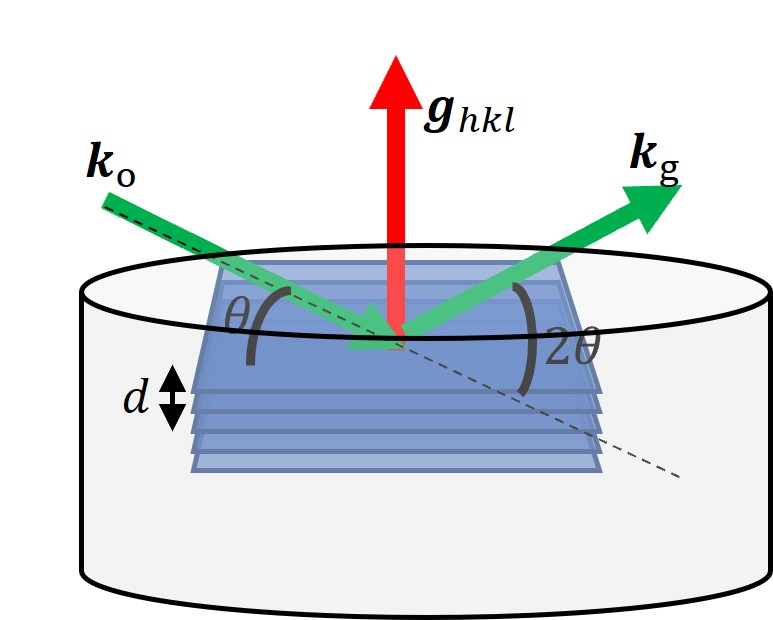
\includegraphics[scale=0.9]{theta_2theta.jpg}
					\caption{$\theta-2\theta$測定における面間隔$d$と$\theta$の関係。赤い矢印は回折に寄与している格子面の法線方向。}
					\label{XRD_theta_2theta}
				\end{minipage}
			\end{figure}
			\newpage
			\begin{figure}[h]
				\centering
				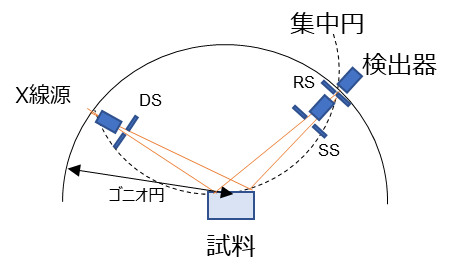
\includegraphics[scale=1.3]{XRD_theta_2theta_光学系.png}
				\caption{集中法光学系}
				\label{集中法光学系}
			\end{figure}

			\subsubsection{Pole figure測定の原理}
			$\theta-2\theta$測定は試料表面に平行な格子面を測定するため、
			結晶面の逆格子ベクトル$\bm{g}_{hkl}$は常に試料の表面に垂直方向を向いている。
			逆格子ベクトル$\bm{g}_{hkl}$の大きさは結晶面の間隔$d$の逆数$1/d$に対応しており、
			$\theta-2\theta$測定は結果的に様々な$d$値の格子面を観測する。
			$\theta-2\theta$測定においても試料の配置を変更するなどによって配向の有無程度は判断可能である。
			しかし配向度などの定量な詳しい評価はPole figure測定などが必要になる。
			
			Pole figure測定(別名:極点測定)は$\theta-2\theta$測定における回折角度$2\theta$を固定し、
			試料を回転、あおりを行い回折強度を測定する手法である。測定する回折面は固定されているため図\ref{極点の測定方法}の通り
			、$\bm{g}_{hkl}$の長さは一定となる。試料を$\alpha$(あおり)と$\beta$(面内回転)という
			2つの優先方位軸を用いて、回折角度一定の半球をスキャンする。
			計測結果は図\ref{極点の測定方法}(B)の通り、極図形を用いて表現する。
			配向度は図\ref{極点の測定方法}(C)の通り、得られた極座標を半径方向に積分し、以下の式\ref{orientation}に基づいて計算される。
			\begin{equation}
				配向度 = \frac{360 - \sum ピークの半値幅 }{360}\times 100
				\label{orientation}
			\end{equation}
			\begin{figure}[h]
				\centering
				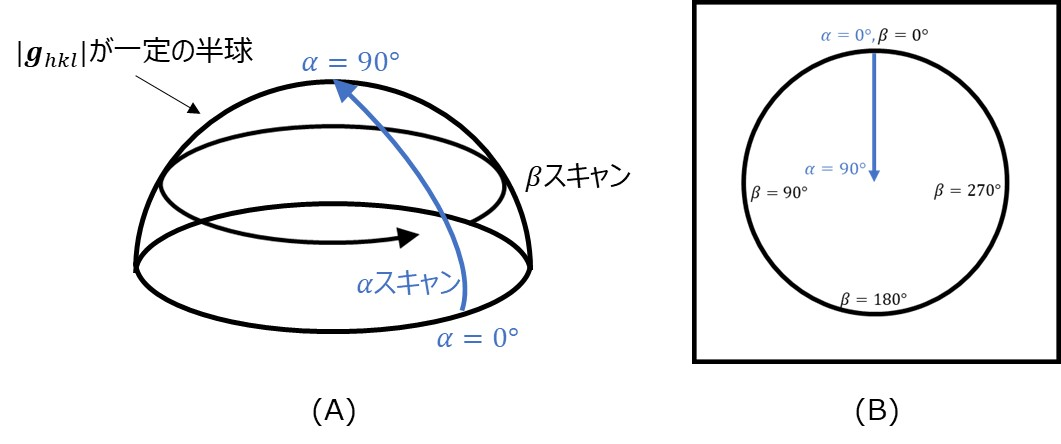
\includegraphics[width=\linewidth]{極点の測定方法.jpg}
				\caption{Pole figure測定の概念図. (A)はスキャン方向. (B)は極図形. (C)は極図形の$\beta$依存性.}
				\label{極点の測定方法}
			\end{figure}
			\newpage
			Pole figure測定には図\ref{Pole_figure_outplane}のアウトプレーンの測定と図\ref{Pole_figure_inplane}のインプレーンの測定が存在する。
			アウトプレーンは試料に対するあおりを試料台を傾けて実現する。
			よって、$\alpha=0^{\circ}$近傍においては試料の側面に入射されてしまうため測定が困難になる。
			結果的にアウトプレーンの想定では$\alpha=0^{\circ}\sim90^{\circ}$の全極点測定は実質不可能である。
			インプレーンのPole figure測定は図\ref{Pole_figure_inplane}の通り、
			試料台を傾けず受光部を傾けてあおり$\alpha$を実現する。
			光学系においては図\ref{XRD_配置}の$2\theta$軸に直行する軸である$2\theta_\chi$軸を利用する。
			インプレーンのPole figure測定で$\alpha=0$は低角で測定する薄膜法を同様の状況であるため、
			薄膜法で使用する光学素子を使用する。例えば、集中光学法では集中発散ビーム(BB)を使用するが
			Pole figure測定では薄膜法で使用される平行ビーム(PB)を使用する。
			本研究においてはPole figure測定が可能であるSmart lab(Rigaku Corporation)を使用した。
			
			\begin{figure}[h]
				\centering
				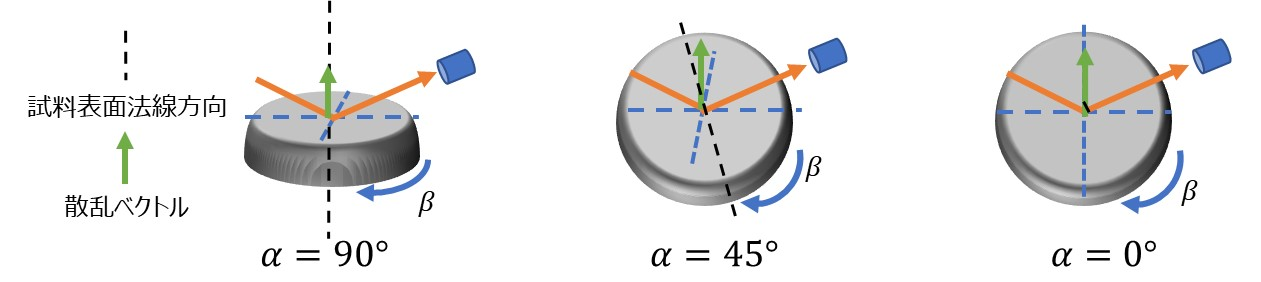
\includegraphics[width=0.9\linewidth]{pole_figure_outplane.jpg}
				\caption{アウトプレーンのPole figure測定}
				\label{Pole_figure_outplane}
			\end{figure}
			\begin{figure}[h]
				\centering
				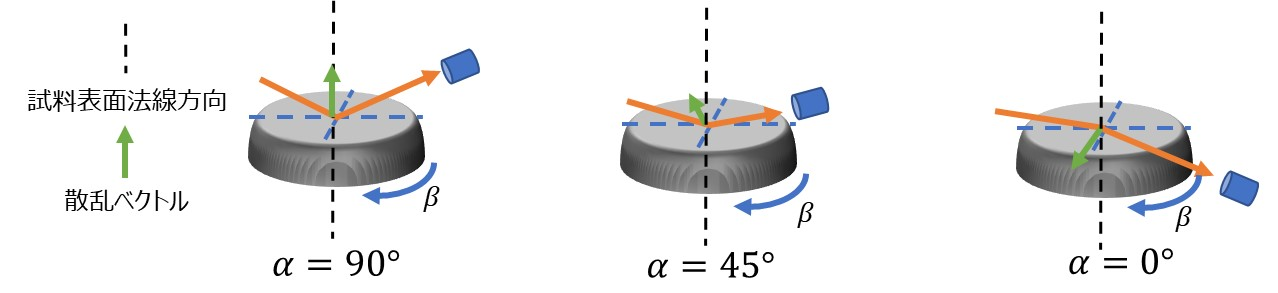
\includegraphics[width=0.9\linewidth]{pole_figure_inplane.jpg}
				\caption{インプレーンのPole figure測定}
				\label{Pole_figure_inplane}
			\end{figure}
			\begin{figure}[h]
				\centering
				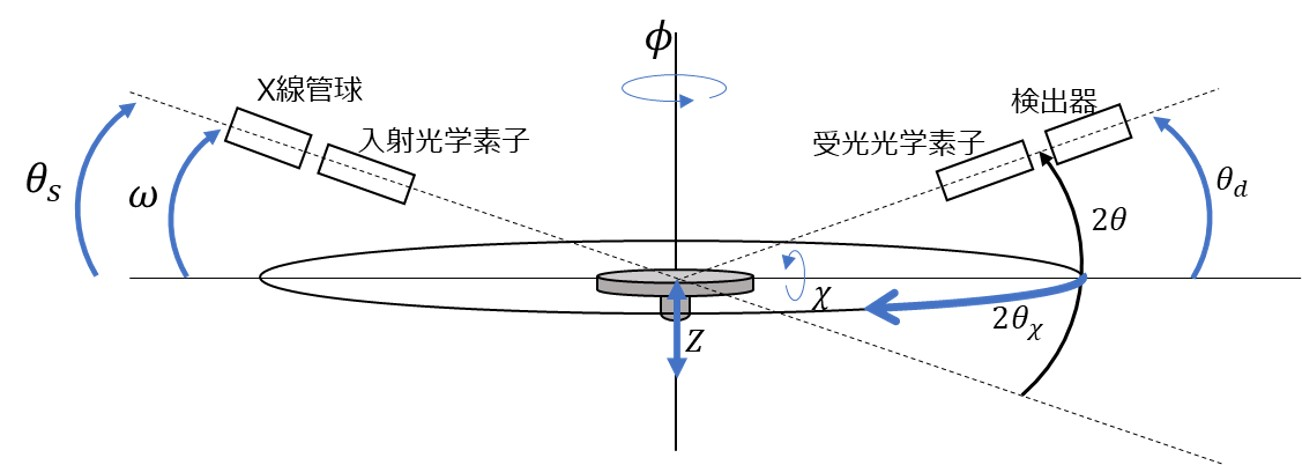
\includegraphics[width=0.9\linewidth]{XRD_配置.jpg}
				\caption{XRDの測定系}
				\label{XRD_配置}
			\end{figure}
			\newpage
			\begin{figure}[h]
				\centering
				
\includegraphics{sora.jpg}
				\caption{Pole figure測定に用いたXRD(Rigaku corportaion)}
				\label{XRD_pole_figure}
			\end{figure}
			\newpage
			\subsection{原子間力顕微鏡(AFM), 圧電応答顕微鏡(PFM)}
			原子間力顕微鏡(AFM)、圧電応答顕微鏡(PFM)はどちらも走査型プローブ顕微鏡(SPM)に属する。
			走査型プローブ顕微鏡(SPM)とは、微小な深針(カンチレバー)で試料をなぞり、
			その形状や物性を観察、計測する顕微鏡の総称である。図\ref{SPM}, \ref{cantilever_photo_detector}
			にSPMの基本構成を示す。SPMに属する顕微鏡は図\ref{SPM}のように
			カンチレバーを試料表面に接触または接近させて、走査中に生じる試料のある物理量の変化を検出する。
			本研究にて用いるSPMは原子間力顕微鏡(AFM)と圧電応答顕微鏡(PFM)のみである。
			この二つにおいては、図\ref{cantilever_photo_detector}のようにそれぞれの物理量変化
			によってカンチレバーがたわみ、そのカンチレバーに照射したレーザーの変位を
			フォトディテクターで計測し、測定対象の物理量変化を測定する。
			つまり、レーザーの変位から物質表面の物性変化をみる。
			原子間力顕微鏡(AFM)はカンチレバーと試料間に生じる原子間力を検出し
			試料表面画像を取得する。圧電応答顕微鏡(PFM)は試料の逆圧電効果に
			よる表面の歪みをカンチレバーの変位として取得し画像化する。
			\begin{figure}[h]
				\centering
				\begin{minipage}{0.45\hsize}
					\centering
					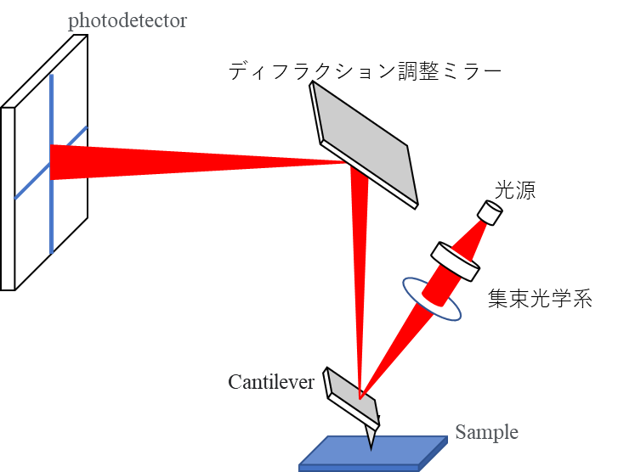
\includegraphics[width=\linewidth]{SPM.png}
					\caption{走査型顕微鏡(SPM)の光学系}
					\label{SPM}
				\end{minipage}
				\begin{minipage}{0.45\hsize}
					\centering
					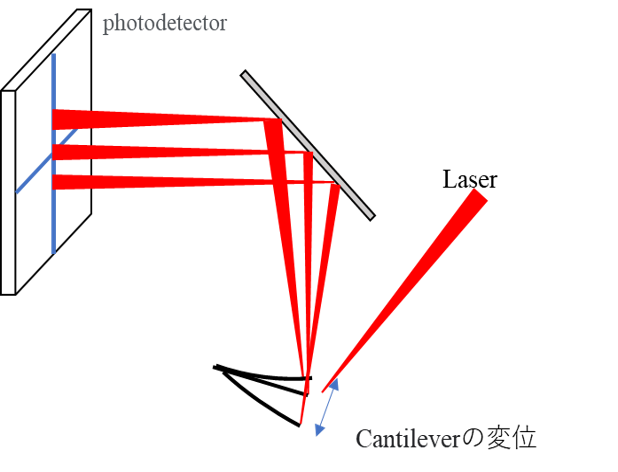
\includegraphics[width=\linewidth]{SPM2.png}
					\caption{CantileverとPhotodetectorの関係}
					\label{cantilever_photo_detector}
				\end{minipage}
			\end{figure}
				\subsubsection{AFM(Atomic Force Microscopy)}
				\begin{figure}[h]
					\centering
					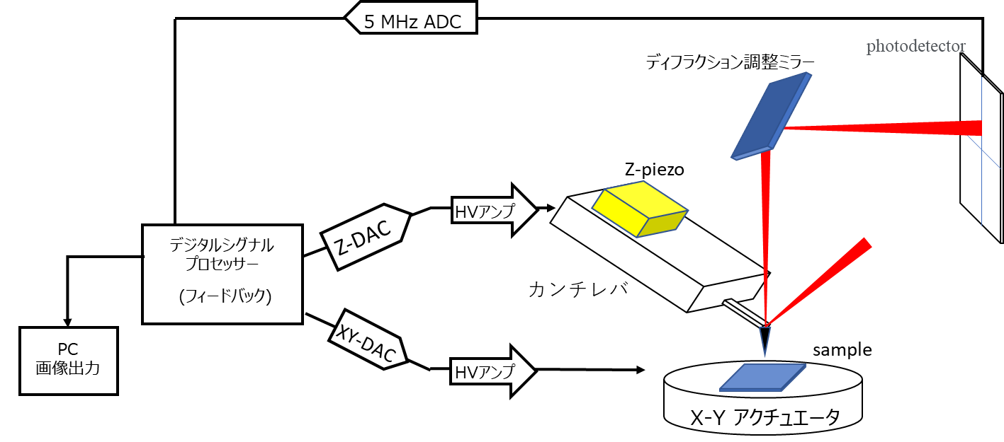
\includegraphics[width=0.8\linewidth]{AFM.png}
					\caption{AFMの信号模式図}
					\label{stracture_of_AFM}
				\end{figure}
				図\ref{stracture_of_AFM}はAFMの信号模式図である。AFMの測定手法にはタッピングモード(ACモード)
				とコンタクトモード(DCモード)がある。タッピングモードは、カンチレバーを内部に存在する圧電素子を用いて
				共振周波数で振動させ、試料表面を断続的に接触させながら走査する。測定対象の表面形状からカンチレバーの振動振幅が変動し、
				画像化する。正確にはカンチレバーを試料表面に近づけると原子間力を検出し、
				この瞬間カンチレバーの振動振幅は小さくなる。この振動振幅の変位をレーザーの変位として取得し、
				この変位分だけ元に戻すようにフィードバックをかけ、Z軸方向をZピエゾで調整する。このZピエゾの変位を画像化し、表面像を得る。
				コンタクトモードはタッピングモードと異なり、
				カンチレバーを振動させずに静的な状態で試料に常に接触させながら試料表面を走査し、
				表面の凹凸に対応したカンチレバーのたわみをレーザーの変位としてフォトディテクターから検出する。
				このレーザーの変位を一定にするようにZピエゾを用いて、フィードバック制御を行う。そのZピエゾの変位を表面形状として画像化する。
				本研究において、AFMを用いた計測はカンチレバーの消耗の観点からタッピングモードで行った。
				\subsubsection{PFM(Piezoresponse Force Microscopy)}
				走査型プローブ顕微鏡(Scanning Prob Microscope, SPM)の一種として圧電応答顕微鏡(Piezoresponse Force Microscopy, PFM)がある。
				圧電応答顕微鏡(PFM)は試料の逆圧電効果による表面の歪みをカンチレバーの変位として取得し画像化する顕微鏡である。
				図\ref{PFMの概念図}のように試料片面基板からカンチレバー間で交流電場を印加する。
				このとき試料の分極方向に依存して、電場の変化に対応した歪みが試料に生じる。
				その歪の大きさはカンチレバーの変位の大きさとして現れ、
				Amplitude像として取得できる。
				\begin{figure}[h]
					\centering
					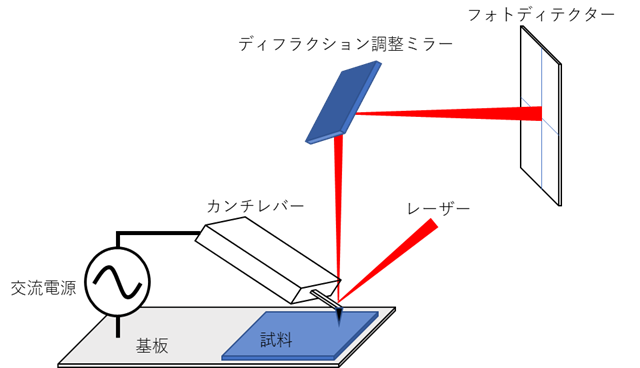
\includegraphics{PFM.png}
					\caption{PFMの概念図}
					\label{PFMの概念図}
				\end{figure}
				\\
				また、図\ref{PFM_phaseの概念図}のように交流電場に対応した試料の歪み方向は試料中の分極方向に依存しているため、
				この分極方向を交流電場と歪みの位相差から解析し、Phase像として取得できる。
				\begin{figure}[h]
					\centering
					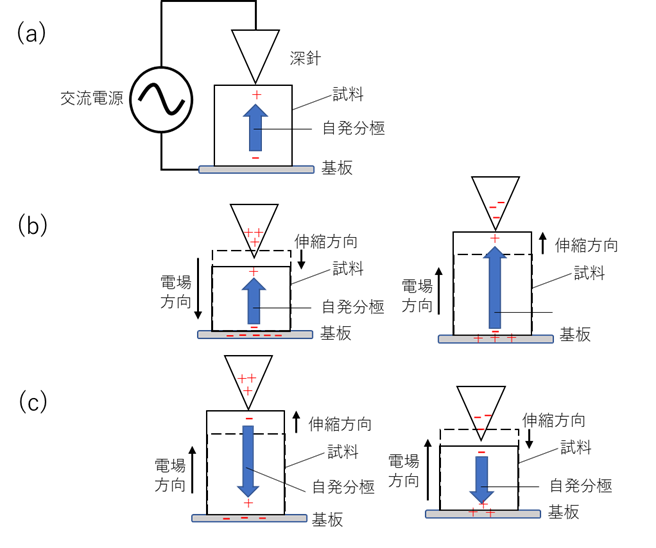
\includegraphics[width=0.8\linewidth]{PFM_phase.png}
					\caption{PFMのPhase像概念図。(a):電場E=0,(b):交流電場と試料の伸縮方向が同位相であるときの自発分極方向,(c):交流電場と試料の伸縮方向が逆位相であるときの自発分極方向}
					\label{PFM_phaseの概念図}
				\end{figure}
				PFMはカンチレバーを試料上に接触させ走査するコンタクトモードで行われる。
				カンチレバーと試料からの相互作用を加味した共振周波数、
				コンタクト周波数でカンチレバーを振動させることで、
				その振動振幅の変化から、より高精度に圧電応答を観察できるようになっている。
				しかし、そのコンタクト周波数は走査中一定に保たれているわけではない。
				なぜならば、走査中の試料表面の形状変化によるカンチレバーの接触面積の違いがコンタクト周波数をシフトさせる要因になる。
				コンタクト周波数のシフトにより、圧電応答によるカンチレバーのたわみ変化の大きさと走査中における試料表面の形状変化によるカンチレバーのたわみ変化がクロストークしてしまい、
				正確な圧電応答や表面像を取得できなくなる。よって測定材料は測定前に表面を平らにする必要がある。
				
				図\ref{PFM_phaseの概念図}は垂直方向のみでの議論である。しかし、図\ref{PFMの概念図}におけるフォトディテクターから分かる通り、
				図\ref{面内と垂直の概念図}の様に試料の面内方向の圧電性の評価も可能である。本研究においてはずり圧電の評価にて使用した。
				\begin{figure}[h]
					\centering
					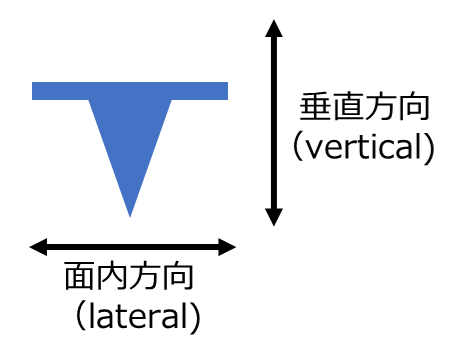
\includegraphics[scale=0.7]{lateral_vertical.png}
					\caption{カンチレバーにおける面内方向(Lateral)と垂直方向(Vertical)の関係}
					\label{面内と垂直の概念図}
				\end{figure}
				\newpage
				生体材料の一つであるコラーゲンの圧電行列は以下の通りである。
				\begin{equation}
					\left(
				\begin{array}{cccccc}
					0&0&0&d_{14}&d_{15}&0 \\
					0&0&0&d_{15}&-d_{14}&0 \\
					d_{31}&d_{31}&d_{33}&0&0&0
				\end{array}\right)
			\end{equation}
				コラーゲン繊維の側面において面内PFM、コラーゲン繊維の断面において垂直PFMを行った報告がある\cite{コラーゲン繊維PFM}。
				このように生体材料の圧電測定においてPFMは頻繁に利用されている。
				\begin{figure}[ht]
					\begin{center}
					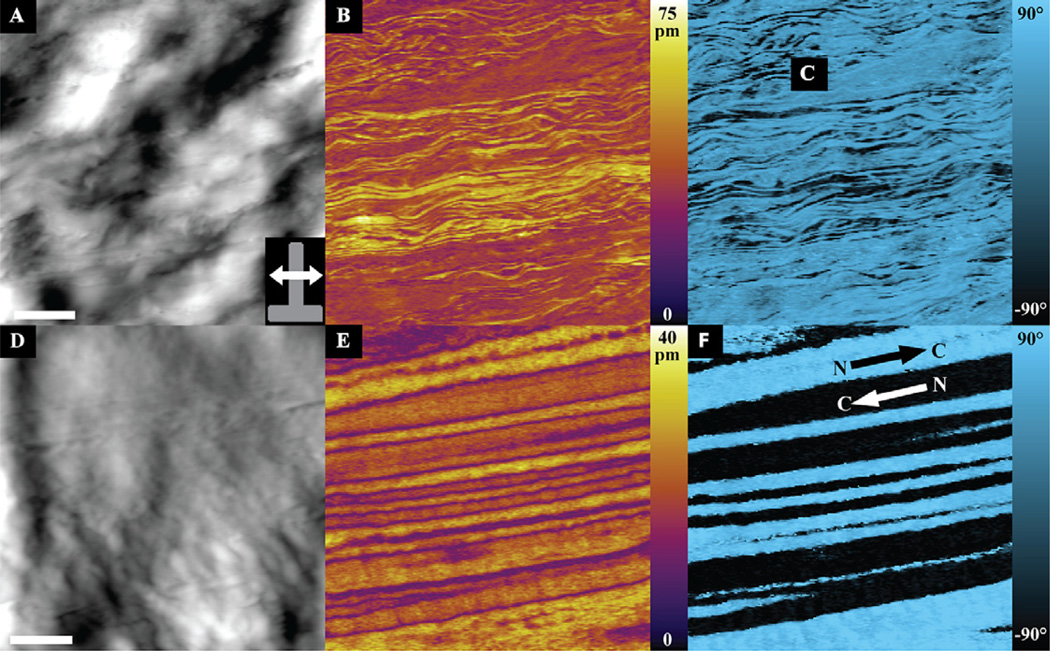
\includegraphics[scale=0.6]{PFM_コラーゲン_側面.jpg}
					\caption{コラーゲン繊維(側面)での面内PFM\cite{コラーゲン繊維PFM}.
					(A)AFM topology(B)面内PFM(C)面内PFMのPhase
					(D)AFM topology(E)面内PFM(F)面内PFMのPhase.
					(A)-(C)のスケールバーは2 {\textmu}m, 
					(D)-(F)のスケールバーは200 nm.}
					\label{PFM_コラーゲン_側面}
					\end{center}
				\end{figure}
				\begin{figure}[h]
					\centering
					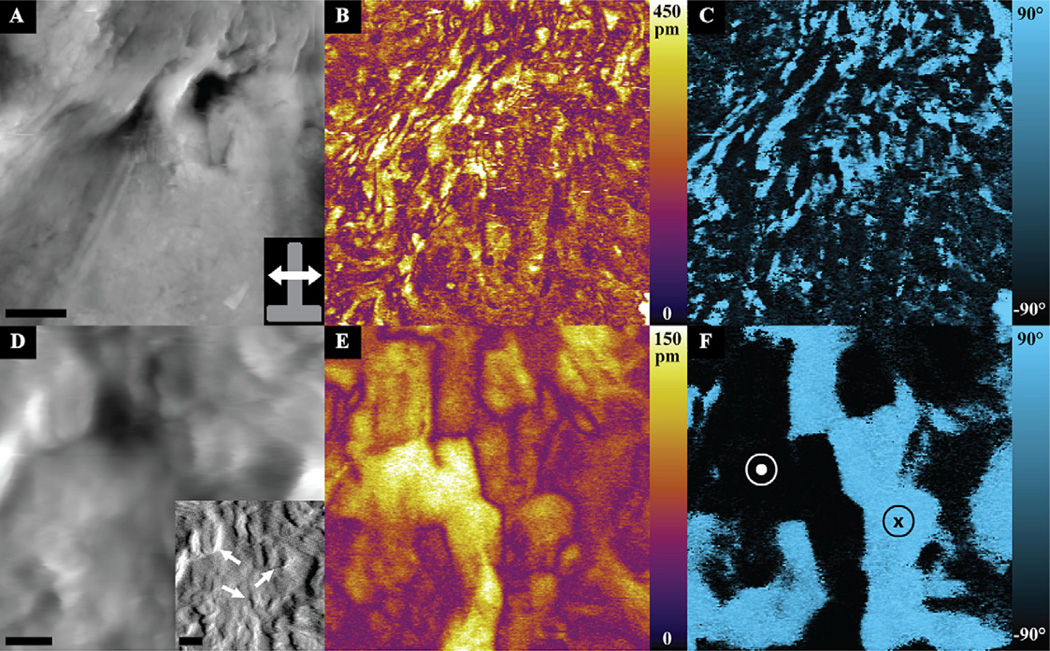
\includegraphics[scale=0.6]{PFM_コラーゲン_断面.jpg}
					\caption{コラーゲン繊維(断面)での垂直PFM\cite{コラーゲン繊維PFM}.
					(A)AFM topology(B)垂直PFM(C)垂直PFMのPhase
					(D)AFM topology(E)垂直PFM(F)垂直PFMのPhase.
					(A)-(C)のスケールバーは2 {\textmu}m, 
					(D)-(F)のスケールバーは200 nm.}
					\label{PFM_コラーゲン_断面}
				\end{figure}
				\newpage
			\subsection{誘電率測定と圧電共鳴法}
			作成したシルクフィブロインフィルムの誘電率はインピーダンスアナライザ
			図\ref{インピーダンスアナライザ}(KEYSIGHT 4294A)を用いて測定した。
			圧電性の評価においては誘電率に現れる圧電性による効果を圧電共鳴法に基づいて評価した。
			\subsubsection{誘電率測定の原理}
			インピーダンスアナライザは自動平衡ブリッジ回路で構成されており図\ref{自動平衡ブリッジ回路}の通りである。
			自動平衡ブリッジ回路は試料に印加される電圧を計測する交流電圧計$V_1$と、
			試料を流れる電流を算出するために用いる交流電圧計$V_2$から構成されている。
			また、交流電圧計$V_1$は四端子測定が行われている。
			図\ref{自動平衡ブリッジ回路}における$L_C$はオペアンプの仮想短絡により0 Vである。
			オペアンプの高インピーダンス特性により、試料を流れる電流$i_x$と$i_r$は等価とみなせる。
			$i_r$は以下の式の通り、交流電圧計$V_2$を用いて計算できる。
			\begin{equation}
				i_r=i_x=-\frac{V_2}{R_r}
			\end{equation}
			試料に印加される電圧$V_1$と試料を流れる電流$i_x$を用いて以下の式のように、
			試料のインピーダンス$Z$を算出できる。
			また、式\ref{impedance}における$R$はレジスタンス、$X$はリアクタンスである。
			\begin{equation}
				Z=\frac{V_1}{i_x}=\frac{V_1}{i_r}=-\frac{V_1}{V_2}R_r = R + j X  
				\label{impedance}
			\end{equation}
			式\ref{impedance}より基準抵抗$R_r$と交流電圧比$V_1/V_2$から求まる。
			また、アドミッタンスはインピーダンスの逆数であるため式\ref{admittance}のように決まる。
			式\ref{admittance}における$G$はコンダクタンス、$B$はサセプタンスである。
			\begin{equation}
				Y= \frac{1}{Z}=-\frac{V_2}{V_1}\frac{1}{R_r} = G + j B
				\label{admittance}
			\end{equation}
			\begin{figure}[h]
				\centering
				\begin{minipage}{0.45\hsize}
					\centering
					
\includegraphics{sora.jpg}
					\caption{KEYSIGHT 4294A}
					\label{インピーダンスアナライザ}
				\end{minipage}
				\begin{minipage}{0.45\hsize}
					\centering
					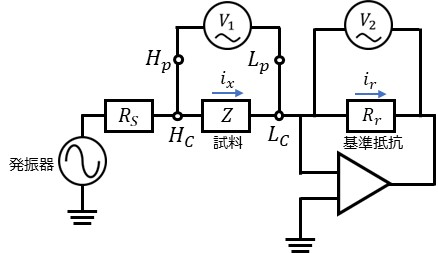
\includegraphics{自動平衡ブリッジ回路.jpg}
					\caption{自動平衡ブリッジ回路}
					\label{自動平衡ブリッジ回路}
				\end{minipage}
			\end{figure}

			測定試料が高インピーダンスな誘電体であり、
			測定する周波数区間が40 Hz -110 MHzであるため、
			測定試料の等価回路として抵抗$R$とコンデンサ$C$の並列モデルを採用する。
			このとき、アドミッタンス$Y_s$は以下のように記述できる。
			\begin{equation}
				Y_s = \frac{1}{R}+j\omega C
				\label{Y_s}
			\end{equation}
			一方、測定試料を理想的なコンデンサとみなすとき、そのアドミッタンスは試料の寸法
			(厚さ$d$, 電極面積$S$)を用いて以下のように求められる。
			\begin{equation}
				Y_p= j \omega C_p = j \omega \varepsilon^{*} \frac{S}{d} = 
				j\omega (\varepsilon'-j\varepsilon'')\frac{S}{d} =
				\omega\varepsilon''\frac{S}{d} + j\omega \varepsilon' \frac{S}{d}
				\label{Y_p}
			\end{equation}
			式\ref{Y_s}の$Y_s$と式\ref{Y_p}の$Y_p$は等価であるため、
			誘電率の実部$\varepsilon'$と虚部$\varepsilon''$は以下のように記述できる。
			\begin{equation}
				\varepsilon' = C \frac{d}{S}
				\label{real_epsilon}
			\end{equation}
			\begin{equation}
				\varepsilon'' = \frac{d}{\omega R S}
				\label{imaginary_epsilon}
			\end{equation}
			これより、インピーダンスアナライザを用いてアドミッタンス$Y$を計測しその実部虚部から、
			抵抗$R$とコンデンサ$C$の値を求めて、式\ref{real_epsilon}と式\ref{imaginary_epsilon}から
			誘電率の実部虚部を計算出来る。圧電性の評価においては誘電率を測定し圧電共鳴法を用いて評価した。
			\subsubsection{圧電共鳴法}

			\newpage
			\subsection{DSC}
	\chapter{結果と考察}
	\chapter{総括}
	\chapter{付録}
	\bibliography{master} %hoge.bibから拡張子を外した名前
	\bibliographystyle{junsrt} %参考文献出力スタイル
	\chapter*{謝辞}
	
\end{document}